% Slides for 2024-08-06
\begin{frame}{Feature extraction and matching - success}
    \centering
    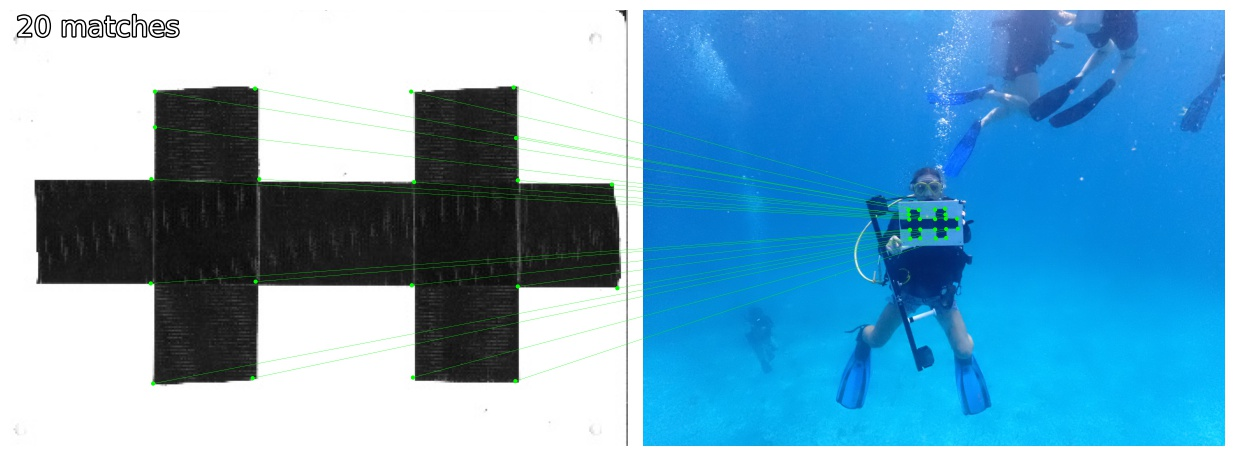
\includegraphics[height=0.7\textheight,width=0.7\textwidth,keepaspectratio]{images/fs_success1.JPG}
    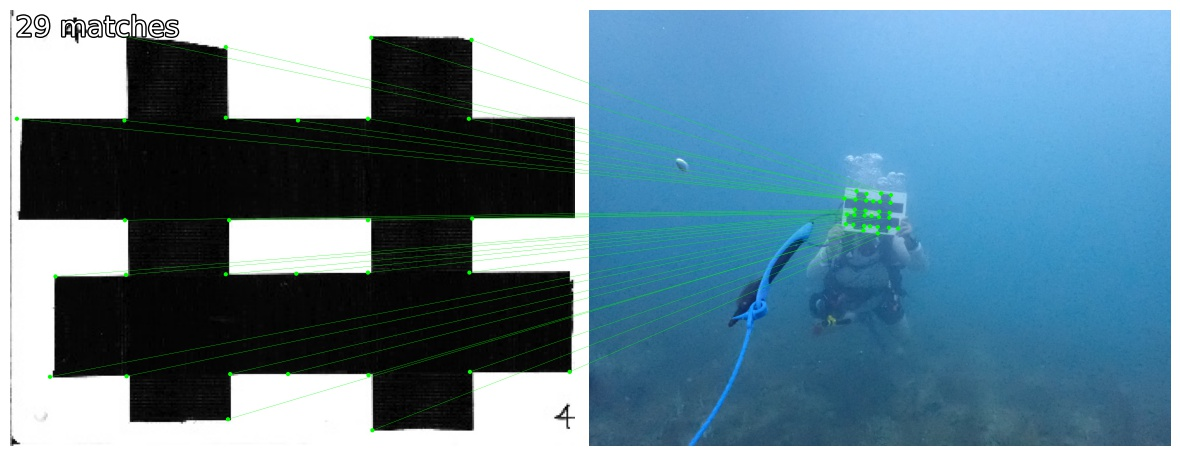
\includegraphics[height=0.7\textheight,width=0.7\textwidth,keepaspectratio]{images/fs_success2.JPG}
\end{frame}

\begin{frame}{Feature extraction and matching - fail}
    \centering
    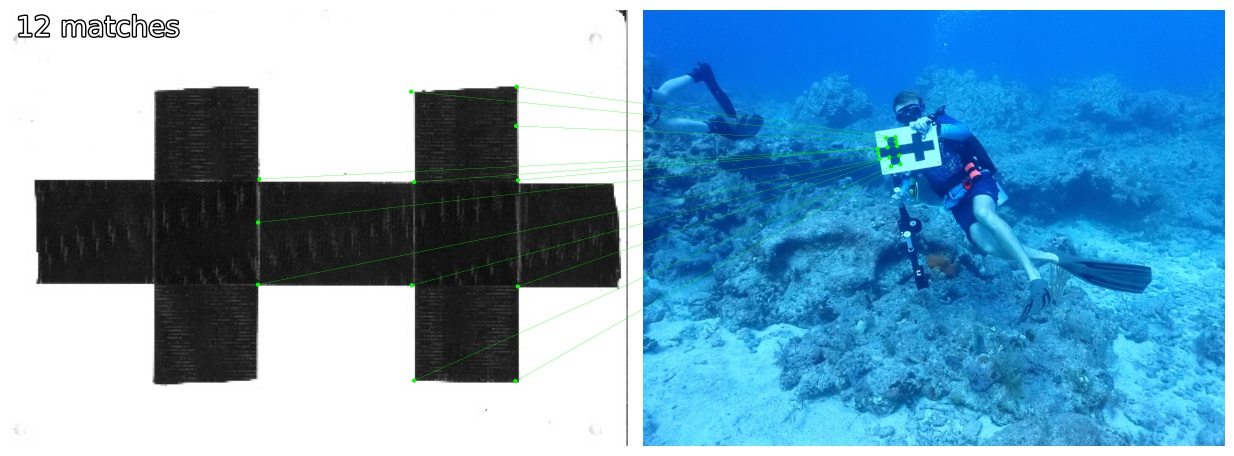
\includegraphics[height=0.7\textheight,width=0.7\textwidth,keepaspectratio]{images/fs_fail1.JPG}
    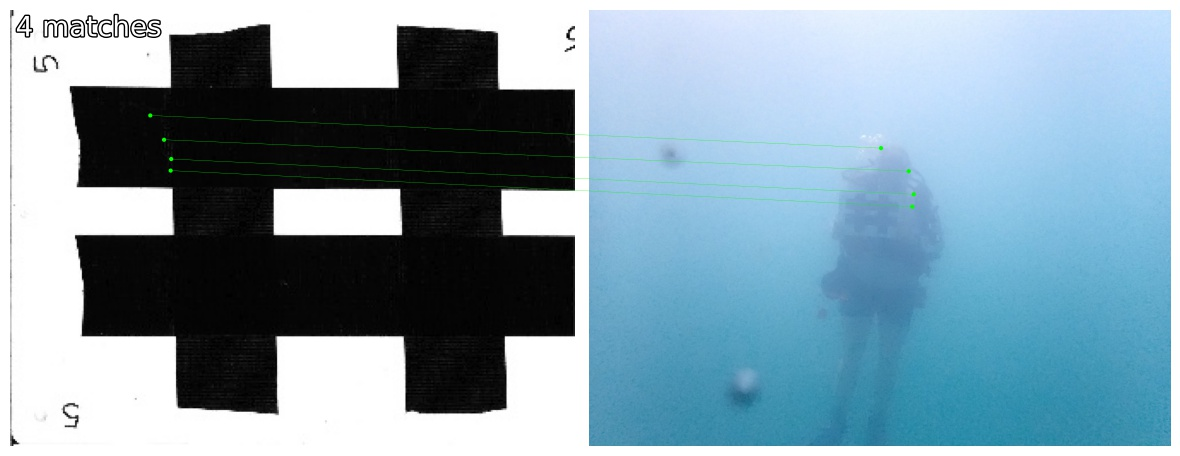
\includegraphics[height=0.7\textheight,width=0.7\textwidth,keepaspectratio]{images/fs_fail2.JPG}
\end{frame}

\begin{frame}{Feature extraction and matching - example use}
    \centering
    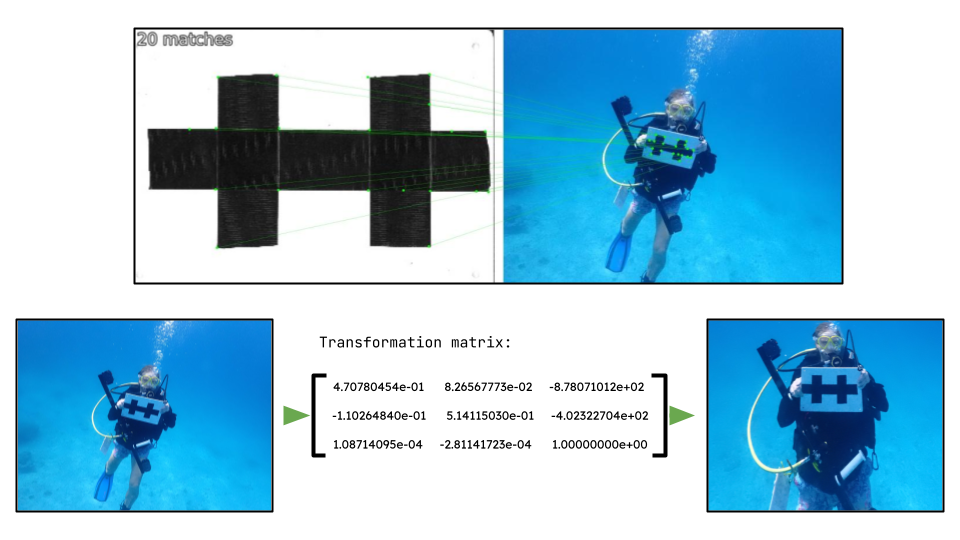
\includegraphics[height=1.0\textheight,width=1.0\textwidth,keepaspectratio]{images/fs_homography_warped.png}
\end{frame}

\begin{frame}{Feature extraction and matching - results} 
    \begin{columns}
        \begin{column}{0.3\textwidth}
            Performance:
            \begin{itemize}
                \item 62/77 algorithm
                \item 57/77 real
            \end{itemize}
        \end{column}
        \begin{column}{0.3\textwidth}
            Without last 10:
            \begin{itemize}
                \item 62/67 algorithm
                \item 57/67 real
            \end{itemize}
        \end{column}
    \end{columns}
\end{frame}